\section{Metodologia}

%\subsection{Equações de fluxo}
%\begin{frame}
%  Em coordenadas radiais, a equação de Richards
%$$
%{\partial \theta \over \partial t} = {1 \over r}{\partial \over \partial r} \left( r K(h) {\partial H \over \partial r} \right)
%$$
%
%e a Equação de Convecção-Dispersão
%
%$$
%r {\partial(\theta C) \over \partial t} = -{\partial \over \partial r} \biggl(r q C \biggr) + {\partial  \over \partial r} \left( r D {\partial C \over \partial r} \right).
%$$
%
%\end{frame}

\subsection{Descrição geral do modelo}
\begin{frame}\frametitle{Características do domínio}

  \begin{tabular}{cl}  
  \begin{tabular}{c}
    \includegraphics[height=2.5cm]{root_zone}\\
    \includegraphics[height=4cm]{domain}
  \end{tabular} &
    \begin{tabular}{l}
    \parbox{0.5\linewidth}{%  change the parbox width as appropiate
      \scriptsize{
	Equação de Richards
	$$
        {\partial \theta \over \partial t} = {1 \over r}{\partial \over \partial r} \left( r K(h) {\partial H \over \partial r} \right)
        $$
	Equação de Convecção-Dispersão
        $$
        r {\partial(\theta C) \over \partial t} = -{\partial \over \partial r} \biggl(r q C \biggr) + {\partial  \over \partial r} \left( r D {\partial C \over \partial r} \right) \\
        $$}

	Condições de contorno em $r_0$:

    \tiny{
      Água:\\
      $T_p$ quando transpiração é potencial\\
      Limitada por K($\theta$) quanto $T_r<1$ \\[0.1cm]
      %$$ K(h) {\partial h \over \partial r} = q_0 = {T_p \over 2 \pi r_0 R z}$$
      Soluto:
      $$ -D(\theta) {\partial C \over \partial r} + q_0 C_0 = q_{s_0} = -{F \over 2\pi r_0 R z}$$
    }

      }
  \end{tabular} 
\end{tabular}
\end{frame}

\begin{frame}\frametitle{Condição de cotorno em $r_0$}

\begin{tabular}{cl}  
  \begin{tabular}{c}
    \centering
    \includegraphics[height=3.5cm]{MM_c}
  \end{tabular} & 
  \begin{tabular}{l}
    \parbox{0.4\linewidth}{ 
      Extração de soluto dependente da concentração de soluto no solo (MM equation) \\[0.1cm]
      $C_{lim}$ e $C_2$ calculados analiticamente (não adiciona novos parâmetros)
    }
  \end{tabular}  \\
  \begin{tabular}{l}
  \parbox{0.5\linewidth}{%  change the parbox width as appropiate
    $$
      F =
      \begin{cases}
	\displaystyle{I_m C_0 \over K_m+C_0}+q_0 C_0, 	&{\rm if }\; C_0 < C_{lim} \\
	I_m, 				 		&{\rm if }\; C_{lim} \leq C_0 \leq C_2 \\
	q_0 C_0, 					&{\rm if }\; C_0 > C_2
      \end{cases}
    $$
  }
  \end{tabular} & 
  \begin{minipage}{5cm}
  Premissas:
    \begin{itemize}
      \item Extração por fluxo de massa $\rightarrow$ passivo
      \item Extração por difusão $\rightarrow$ ativo
      \item Parâmetro $I_m$ $\rightarrow$ demanda da planta por soluto
      \item Em $C_{lim}$ a extração é limitada pelo fluxo de soluto
    \end{itemize}
  \end{minipage}
  \\

\end{tabular}

\end{frame}

\subsection{Implementação numérica da ECD}
\begin{frame}
  \begin{block}{Discretização}
  \begin{itemize}
    \item Solução implícita (backward Euler method)
    \item Discretização do espaço $\rightarrow$ não-constante ($\Delta_r$ crescente) $\rightarrow$ maior precisão (malha mais fina) na zona de maior variação de fluxos
    \item Discretização do tempo $\rightarrow$ variável (de acordo com o número de iterações)
  \end{itemize}
  \end{block} \pause
  
  \begin{block}{Modelo proposto}
    \begin{itemize}
      \item Extração não-linear (MM Equation) e linear (baseada em MM) em $r_0$\\
	\begin{tabular}{ll}
	  \multirow{8}{*}{\includegraphics[height=3.cm]{MM_LNL}} & \\
								  & \\
								  & $F = \displaystyle{I_m C_0 \over K_m + C_0} + q_0 C_0 $ \\
								  & \\
								  & \\
								  & $F = \beta C_0 = {2 I_m \over K_m \pm \left( {K_m}^2 + 4{I_m K_m / q_0} \right)^{1/2}} C_0 $ \\
								  & \\
								  & \\
	\end{tabular}
    \end{itemize}
  \end{block}
\end{frame}

\subsection{Implementação}
\begin{frame}\frametitle{Outros modelos (comparação)}
  Algoritmo numérico da solução analítica de \cite{willigen1} $\rightarrow$ Extração de soluto em taxa constante \\[0.5cm]

  Algoritmo da solução numérica de \cite{liersolute} $\rightarrow$ Sem extração de soluto\\[.5cm]

  Algoritmo da solução analítica de \cite{cushman} $\rightarrow$ Extração de soluto dependente da concentração no solo

\end{frame}

\subsection{Cenários de simulação, entradas e saídas do modelo}
\begin{frame}[fragile]
\long\def\pmb#1{\setbox0=\hbox{#1}\copy0\kern-\wd0%
\kern0.02em\raise0.02ex\copy0\kern-\wd0\kern0.02em\box0}
\newcommand*{\myalign}[2]{\multicolumn{1}{#1}{#2}}	% change align of just one cell

\begin{block}{Cenários}
{\tiny
\begin{tabular}{cccccc}
\hline
\myalign{l}{\bf Scenario} & \pmb{$R$} & \pmb{$C_{ini}$} & \pmb{$T_p$} & {\bf Soil} & {\bf Ion}  \\ \hline 
1         & M                   & H            	                & H	                              &	Loam       &  K$^+$    \cr
2         & M                   & H            	                & L                        &	Loam       & K$^+$     \cr
3         & M                   & L           	                & H	                      &	Loam       & K$^+$     \cr
4         & H                   & H            	                & H	                      &	Loam       & K$^+$     \cr
5         & L                   & H            	                & H	                      &	Loam       & K$^+$     \cr
6         & M                   & H            	                & H	                      &	Sand                & K$^+$     \cr
7         & M                   & H            	                & H	                      &	Clay                & K$^+$     \cr
8         & M                   & H            	                & H	                      &	Loam                &  NO$^-_3$   \\ \hline
\end{tabular}\\[.2cm]
$R$: densidade radicular\\
$C_{ini}$: concentração inicial de soluto no solo\\
$T_p$: transpiração potencial
}
\end{block}
\begin{block}{Parametros de Entradas}
  Solo, planta e atmosfera.
\end{block}

\begin{block}{Saídas}
  Concentrações de soluto ($C(r)$, $C_0(t)$), potenciais ($h$, $h_pi$, $H$) e fluxos ($q(r)$, $q_0(t)$, $q_s(r)$, $q_{s_0}(t)$).
\end{block}

\end{frame}

\subsection{Outras análises}
\begin{frame}
  \begin{block}{Diferença entre a solução linear e a não-linear}
    $$
    \delta_C  = {\sum_{x=1}^{x_{end}} C\!L_x - C\!N\!L_x \over \sum_{x=1}^{x_{end}} C\!L_x}
    $$
    $$
    \delta_{Ac} = {\sum_{t=1}^{t_{end}} AcL_t - AcN\!L_t \over \sum_{t=1}^{t_{end}} AcL_t}
    $$

    Saídas Analisadas: $C(r)$, $C_0(t)$ e $Ac(t)$ (também no teste U).
  \end{block}

  \pause
  \begin{block}{Análise de sensibilidade}
    Sensibilidade parcial relativa.
    $$
    \eta = {dY/Y \over dP/P}\
    $$
    \\[.2cm]
    Parâmetros que sofreram variação ($dP/P = 0.01$):\\
    $I_m$, $K_m$\\
    $\alpha$, $n$, $\lambda$, $K_s$, $\theta_r$, $\theta_s$\\[.2cm]

    Saídas analisadas:\\
    $t_{end}$, $h_\pi$, $h$, $\overline{h_\pi}$, $\overline{h}$, $Ac$ 

  \end{block}
\end{frame}

